% Options for packages loaded elsewhere
\PassOptionsToPackage{unicode}{hyperref}
\PassOptionsToPackage{hyphens}{url}
%
\documentclass[
  ignorenonframetext,
]{beamer}
\usepackage{pgfpages}
\setbeamertemplate{caption}[numbered]
\setbeamertemplate{caption label separator}{: }
\setbeamercolor{caption name}{fg=normal text.fg}
\beamertemplatenavigationsymbolsempty
% Prevent slide breaks in the middle of a paragraph
\widowpenalties 1 10000
\raggedbottom
\setbeamertemplate{part page}{
  \centering
  \begin{beamercolorbox}[sep=16pt,center]{part title}
    \usebeamerfont{part title}\insertpart\par
  \end{beamercolorbox}
}
\setbeamertemplate{section page}{
  \centering
  \begin{beamercolorbox}[sep=12pt,center]{part title}
    \usebeamerfont{section title}\insertsection\par
  \end{beamercolorbox}
}
\setbeamertemplate{subsection page}{
  \centering
  \begin{beamercolorbox}[sep=8pt,center]{part title}
    \usebeamerfont{subsection title}\insertsubsection\par
  \end{beamercolorbox}
}
\AtBeginPart{
  \frame{\partpage}
}
\AtBeginSection{
  \ifbibliography
  \else
    \frame{\sectionpage}
  \fi
}
\AtBeginSubsection{
  \frame{\subsectionpage}
}
\usepackage{lmodern}
\usepackage{amssymb,amsmath}
\usepackage{ifxetex,ifluatex}
\ifnum 0\ifxetex 1\fi\ifluatex 1\fi=0 % if pdftex
  \usepackage[T1]{fontenc}
  \usepackage[utf8]{inputenc}
  \usepackage{textcomp} % provide euro and other symbols
\else % if luatex or xetex
  \usepackage{unicode-math}
  \defaultfontfeatures{Scale=MatchLowercase}
  \defaultfontfeatures[\rmfamily]{Ligatures=TeX,Scale=1}
\fi
% Use upquote if available, for straight quotes in verbatim environments
\IfFileExists{upquote.sty}{\usepackage{upquote}}{}
\IfFileExists{microtype.sty}{% use microtype if available
  \usepackage[]{microtype}
  \UseMicrotypeSet[protrusion]{basicmath} % disable protrusion for tt fonts
}{}
\makeatletter
\@ifundefined{KOMAClassName}{% if non-KOMA class
  \IfFileExists{parskip.sty}{%
    \usepackage{parskip}
  }{% else
    \setlength{\parindent}{0pt}
    \setlength{\parskip}{6pt plus 2pt minus 1pt}}
}{% if KOMA class
  \KOMAoptions{parskip=half}}
\makeatother
\usepackage{xcolor}
\IfFileExists{xurl.sty}{\usepackage{xurl}}{} % add URL line breaks if available
\IfFileExists{bookmark.sty}{\usepackage{bookmark}}{\usepackage{hyperref}}
\hypersetup{
  pdftitle={Tema 11 - Introducción a distribuciones de probabilidad},
  pdfauthor={Juan Gabriel Gomila \& María Santos},
  hidelinks,
  pdfcreator={LaTeX via pandoc}}
\urlstyle{same} % disable monospaced font for URLs
\newif\ifbibliography
\usepackage{longtable,booktabs}
\usepackage{caption}
% Make caption package work with longtable
\makeatletter
\def\fnum@table{\tablename~\thetable}
\makeatother
\usepackage{graphicx,grffile}
\makeatletter
\def\maxwidth{\ifdim\Gin@nat@width>\linewidth\linewidth\else\Gin@nat@width\fi}
\def\maxheight{\ifdim\Gin@nat@height>\textheight\textheight\else\Gin@nat@height\fi}
\makeatother
% Scale images if necessary, so that they will not overflow the page
% margins by default, and it is still possible to overwrite the defaults
% using explicit options in \includegraphics[width, height, ...]{}
\setkeys{Gin}{width=\maxwidth,height=\maxheight,keepaspectratio}
% Set default figure placement to htbp
\makeatletter
\def\fps@figure{htbp}
\makeatother
\setlength{\emergencystretch}{3em} % prevent overfull lines
\providecommand{\tightlist}{%
  \setlength{\itemsep}{0pt}\setlength{\parskip}{0pt}}
\setcounter{secnumdepth}{-\maxdimen} % remove section numbering

\title{Tema 11 - Introducción a distribuciones de probabilidad}
\author{Juan Gabriel Gomila \& María Santos}
\date{}

\begin{document}
\frame{\titlepage}

\hypertarget{conceptos-buxe1sicos}{%
\section{Conceptos básicos}\label{conceptos-buxe1sicos}}

\begin{frame}{Experimento aleatorio}
\protect\hypertarget{experimento-aleatorio}{}

Experimento aleatorio. Experimento que efectuado en las mismas
condiciones puede dar lugar a resultados diferentes

Suceso elemental. Cada uno de los posibles resultados del experimento
aleatorio

Espacio muestral. Conjunto \(\Omega\) formado por todos los sucesos
elementales del experimento aleatorio

\textbf{Ejemplo}

Lanzar una moneda es un experimento aleatorio

Los sucesos elementales son: sacar cara (\(C\)) y sacar cruz (\(+\))

El espacio muestral de este experimento aleatorio es
\(\Omega = \{C,+\}\)

\end{frame}

\begin{frame}{Sucesos}
\protect\hypertarget{sucesos}{}

Suceso. Subconjunto del espacio muestral

Suceso total o seguro. \(\Omega\)

Suceso vacío o imposible. \(\emptyset\)

\textbf{Ejemplo}

Lanzar un dado es un experimento aleatorio

Algunos sucesos podrían ser: sacar número par (\(\{2,4,6\}\)), sacar
mayor que 4 (\(\{5,6\}\)), sacar número múltiplo de 3
(\(\{3,6\}\))\ldots{}

El suceso total de este experimento aleatorio es
\(\Omega = \{1,2,3,4,5,6\}\)

Un ejemplo de suceso imposible de este experimento aleatorio es
\(\emptyset = \{7\}\) (sacar 7)

\end{frame}

\begin{frame}{Sucesos}
\protect\hypertarget{sucesos-1}{}

Operaciones con sucesos. Sean \(A,B\subseteq \Omega\) sucesos. Entonces,

\begin{itemize}
\tightlist
\item
  \(A\cup B\) es el suceso unión (resultados pertenecen a \(A\), o a
  \(B\), o a ambos)
\item
  \(A\cap B\) es el suceso intersección (resultados pertenecen a \(A\) y
  \(B\))
\item
  \(A^c\) es el suceso complementario (resultados que no pertenecen a
  \(A\))
\item
  \(A-B = A\cap B^c\) es el suceso diferencia (resultados que pertenecen
  a \(A\) pero no a \(B\))
\end{itemize}

Sucesos incompatibles. Si \(A\cap B = \emptyset\)

\end{frame}

\begin{frame}{Probabilidad}
\protect\hypertarget{probabilidad}{}

Probabilidad de un suceso. Número entre 0 y 1 (ambos incluidos) que mide
la expectativa de que se dé este suceso

\textbf{Ejemplo}

\begin{itemize}
\tightlist
\item
  La probabilidad de sacar un 6 al lanzar un dado estándar no trucado es
  \(\frac{1}{6}\)
\item
  La probabilidad de sacar un 6 al lanzar un dado de 4 caras es \(0\)
\item
  La probabilidad de sacar un 6 al lanzar un dado de 20 caras es
  \(\frac{1}{20}\)
\end{itemize}


\includegraphics{Imgs/dado.png}

\end{frame}

\begin{frame}{Probabilidad}
\protect\hypertarget{probabilidad-1}{}

Probabilidad. Sea \(\Omega\) el espacio muestral de un experimento
aleatorio. Suponiendo que \(\Omega\) es \textbf{finito}, una
probabilidad sobre \(\Omega\) es una aplicación
\[p: \mathcal{P}(\Omega)\longrightarrow [0,1]\] que satisface

\begin{itemize}
\tightlist
\item
  \(0\le p(A)\le 1 \ \forall A\in\mathcal{P}(\Omega)\)
\item
  \(p(\Omega) = 1\)
\item
  Si \(\{A_1,\dots,A_n\}\) son sucesos incompatibles dos a dos
  (\(A_i\cap A_j=\emptyset \ \forall i\ne j\)), entonces
  \[p(A_1\cup\cdots \cup A_n)=p(A_1)+\cdots+p(A_n)\]
\end{itemize}

Notación: Si \(a\in\Omega\), escribiremos \(p(a)\) en vez de
\(p(\{a\})\)

\end{frame}

\hypertarget{variables-aleatorias}{%
\section{Variables aleatorias}\label{variables-aleatorias}}

\begin{frame}{Variable aleatoria}
\protect\hypertarget{variable-aleatoria}{}

Variable aleatoria. Una variable aleatoria (v.a.) sobre \(\Omega\) es
una aplicación \[X: \Omega\longrightarrow \mathbb{R}\] que asigna a cada
suceso elemental \(\omega\) un número real \(X(\omega)\)

Puede entenderse como una descripción numérica de los resultados de un
experimento aleatorio

Dominio de una variable aleatoria. \(D_X\), es el conjunto de los
valores que puede tomar

\end{frame}

\begin{frame}{Sucesos de variables aleatorias}
\protect\hypertarget{sucesos-de-variables-aleatorias}{}

Una variable aleatoria puede definir sucesos, de los cuales queremos
conocer la probabilidad \(p\)

\begin{itemize}
\tightlist
\item
  \(p(X=a) = p(\{\omega\in\Omega \ |\  X(\omega) = a\})\)
\item
  \(p(X<b) = p(\{\omega\in\Omega \ |\  X(\omega) < b\})\)
\item
  \(p(X\le b) = p(\{\omega\in\Omega \ |\  X(\omega) \le b\})\)
\item
  \(p(a<X) = p(\{\omega\in\Omega \ |\  a<X(\omega)\})\)
\item
  \(p(a\le X) = p(\{\omega\in\Omega \ |\  a\le X(\omega)\})\)
\item
  \(p(a\le X\le b) = p(\{\omega\in\Omega \ |\  a\le X(\omega) \le b\})\)
\item
  \(p(a< X< b) = p(\{\omega\in\Omega \ |\  a< X(\omega) < b\})\)
\item
  \(p(X\in A) = p(\{\omega\in\Omega \ |\  X(\omega)\in A\})\)
\end{itemize}

\end{frame}

\begin{frame}{Función de distribución}
\protect\hypertarget{funciuxf3n-de-distribuciuxf3n}{}

Función de distribución de la v.a. \(X\). Es una función
\[F:\mathbb{R}\longrightarrow [0,1]\] definida por \(F(x)=p(X\le x)\)

Sea \(F\) una función de distribución de una v.a. \(X\) y digamos
\[F(a^-)=\lim_{x\rightarrow a^-}F(x)\]

\begin{itemize}
\tightlist
\item
  \(p(X\le a)=F(a)\)
\item
  \(p(X<a)=\lim_{b\rightarrow a,\  b<a}p(X\le b) = \lim_{b\rightarrow a,\  b<a} F(b) = F(a^-)\)
\item
  \(p(X=a) = p(X\le a)-p(X<a)=F(a)-F(a^-)\)
\item
  \(p(a\le X\le b) = p(X\le b)-p(X< a)=F(b)-F(a^-)\)
\end{itemize}

\end{frame}

\begin{frame}{Cuantiles}
\protect\hypertarget{cuantiles}{}

Cuantil de orden \(p\) de una v.a. \(X\). Es el \(x_p\in\mathbb{R}\) más
pequeño tal que \(F(x_p)\ge p\)

Nótese que la mediana es el cuantil de orden 0.5

\end{frame}

\hypertarget{variables-aleatorias-discretas}{%
\section{Variables aleatorias
discretas}\label{variables-aleatorias-discretas}}

\begin{frame}{Variable aleatoria discreta}
\protect\hypertarget{variable-aleatoria-discreta}{}

Variable aleatoria discreta. Una v.a.
\(X:\Omega\longrightarrow \mathbb{R}\) es discreta cuando \(D_X\) es
finito o un subconjunto de \(\mathbb{N}\)

Función de probabilidad. Es la función
\(f:\mathbb{R}\longrightarrow[0,1]\) definida por \[f(x) = p(X=x)\]

Nótese que \(f(x)=0\) si \(x\not\in D_X\). Por tanto, interpretaremos la
función de probabilidad como la función \[f:D_X\longrightarrow [0,1]\]

\end{frame}

\begin{frame}{Esperanza}
\protect\hypertarget{esperanza}{}

Esperanza de una v.a. discreta. Sea \(f:D_X\longrightarrow[0,1]\) la
función de probabilidad de \(X\), entonces la esperanza respecto de la
función de probabilidad es la suma ponderada de los elementos de
\(D_X\), multiplicando cada elemento \(x\) de \(D_X\) por su
probabilidad, \[E(X) = \sum_{x\in D_X}x\cdot f(x)\]

Si \(g:D_X\longrightarrow \mathbb{R}\) es una aplicación
\[E(g(X))=\sum_{x\in D_X}g(x)\cdot f(x)\]

\end{frame}

\begin{frame}{Varianza}
\protect\hypertarget{varianza}{}

Varianza de una v.a. discreta. Sea \(f:D_X\longrightarrow[0,1]\) la
función de probabilidad de \(X\), entonces la varianza respecto de la
función de probabilidad es el valor esperado de la diferencia al
cuadrado entre \(X\) y su valor medio \(E(X)\),
\[Var(X)= E((X-E(X))^2) \]

La varianza mide como de variados son los resultados de \(X\) respecto
de la media

\textbf{Ejercicio.} Demostrar la siguiente igualdad.
\[Var(X)= E(X^2)-(E(X))^2\]

\end{frame}

\begin{frame}{Varianza}
\protect\hypertarget{varianza-1}{}

Si \(X\) es una v.a. discreta y \(g:D_X\longrightarrow \mathbb{R}\) una
función, \[Var(g(X))=E((g(X)-E(g(X)))^2)=E(g(X)^2)-(E(g(X)))^2\]

\end{frame}

\begin{frame}{Desviación típica}
\protect\hypertarget{desviaciuxf3n-tuxedpica}{}

Desviación típica de una v.a. discreta. Sea
\(f:D_X\longrightarrow[0,1]\) la función de probabilidad de \(X\),
entonces la desviación típica respecto de la función de probabilidad es
\[\sigma(X)=\sqrt{Var(X)}\]

Las unidades de la varianza son las de \(X\) al cuadrado. En cambio, las
de la desviación típica son las mismas unidades que las de \(X\)

Si \(X\) es una v.a. discreta y \(g:D_X\longrightarrow \mathbb{R}\) una
función, \[\sigma(g(X))=\sqrt{Var(g(X))}\]

\end{frame}

\hypertarget{distribuciones-de-probabilidad}{%
\section{Distribuciones de
probabilidad}\label{distribuciones-de-probabilidad}}

\begin{frame}{Distribución de probabilidad}
\protect\hypertarget{distribuciuxf3n-de-probabilidad}{}

\href{https://es.wikipedia.org/wiki/Distribución_de_probabilidad}{Distribución
de probabilidad}. En teoría de la probabilidad y estadística, la
distribución de probabilidad de una variable aleatoria es una función
que asigna a cada suceso definido sobre la variable la probabilidad de
que dicho suceso ocurra.

\end{frame}

\begin{frame}[fragile]{Distribuciones en \texttt{R}}
\protect\hypertarget{distribuciones-en-r}{}

Dada cualquier variable aleatoria, \texttt{va}, \texttt{R} nos da cuatro
funciones para poder trabajar con ellas:

\begin{itemize}
\tightlist
\item
  \texttt{dva(x,...)}: Función de densidad o de probabilidad \(f(x)\) de
  la variable aleatoria para el valor \(x\) del dominio de definición.
\item
  \texttt{pva(x,...)}: Función de distribución \(F(x)\) de la variable
  aleatoria para el valor \(x\) del dominio de definición.
\item
  \texttt{qva(p,...)}: Cuantil \(p\)-ésimo de la variable aleatoria (el
  valor de \(x\) más pequeño tal que \(F(x)\geq p\)).
\item
  \texttt{rva(n,...)}: Generador de \(n\) observaciones siguiendo la
  distribución de la variable aleatoria.
\end{itemize}

\end{frame}

\begin{frame}[fragile]{Distribuciones en \texttt{Python}}
\protect\hypertarget{distribuciones-en-python}{}

Dada cualquier variable aleatoria, en \texttt{Python} tenemos las mismas
cuatro funciones, sin que su nombre dependa de la misma:

\begin{itemize}
\tightlist
\item
  \texttt{pmf(k,...)} o \texttt{pdf(x,...)}: Función de probabilidad
  \(f(k)\) o de densidad \(f(x)\) de la variable aleatoria para los
  valores \(k\) o \(x\) del dominio.
\item
  \texttt{cdf(x,...)}: Función de distribución \(F(x)\) de la variable
  aleatoria para el valor \(k\) del dominio.
\item
  \texttt{ppf(p,...)}: Cuantil \(p\)-ésimo de la variable aleatoria (el
  valor de \(x\) más pequeño tal que \(F(x)\geq p\)).
\item
  \texttt{rvs(size,...)}: Generador de \(size\) observaciones siguiendo
  la distribución de la variable aleatoria.
\end{itemize}

También vale la pena conocer la función
\texttt{stats(moments=\textquotesingle{}mvsk\textquotesingle{})} que nos
devuelve cuatro valores con los estadísticos de la media \texttt{m}, la
varianza \texttt{v}, el sesgo \texttt{s} y la curtosis \texttt{k} de la
distribución.

\end{frame}

\hypertarget{distribuciones-discretas-muxe1s-conocidas}{%
\section{Distribuciones discretas más
conocidas}\label{distribuciones-discretas-muxe1s-conocidas}}

\begin{frame}{Distribuciones discretas}
\protect\hypertarget{distribuciones-discretas}{}

\begin{itemize}
\tightlist
\item
  \href{https://es.wikipedia.org/wiki/Distribución_de_Bernoulli}{Bernoulli}
\item
  \href{https://es.wikipedia.org/wiki/Distribución_binomial}{Binomial}
\item
  \href{https://es.wikipedia.org/wiki/Distribución_geométrica}{Geométrica}
\item
  \href{https://es.wikipedia.org/wiki/Distribución_hipergeométrica}{Hipergeométrica}
\item
  \href{https://es.wikipedia.org/wiki/Distribución_de_Poisson}{Poisson}
\item
  \href{https://es.wikipedia.org/wiki/Distribución_binomial_negativa}{Binomial
  Negativa}
\end{itemize}

\end{frame}

\begin{frame}{Distribución de Bernoulli}
\protect\hypertarget{distribuciuxf3n-de-bernoulli}{}

Si \(X\) es variable aleatoria que mide el ``número de éxitos'' y se
realiza un único experimento con dos posibles resultados (éxito, que
toma valor 1, o fracaso, que toma valor 0), diremos que \(X\) se
distribuye como una Bernoulli con parámetro \(p\)

\[X\sim \text{Be}(p)\]

donde \(p\) es la probabilidad de éxito y \(q = 1-p\) es la probabilidad
de fracaso.

\begin{itemize}
\tightlist
\item
  El \textbf{dominio} de \(X\) será \(D_X = \{0,1\}\)
\item
  La \textbf{función de probabilidad} vendrá dada por
  \[f(k) = p^k(1-p)^{1-k} =  \left\{
  \begin{array}{rl}
     p & \text{si } k=1 
  \\ 1-p & \text{si } k=0
  \\ 0 & \text{en cualquier otro caso}
  \end{array}
  \right.\]
\end{itemize}

\end{frame}

\begin{frame}{Distribución de Bernoulli}
\protect\hypertarget{distribuciuxf3n-de-bernoulli-1}{}

\begin{itemize}
\tightlist
\item
  La \textbf{función de distribución} vendrá dada por \[F(x) = \left\{
  \begin{array}{rl}
     0 & \text{si } x<0 
  \\ 1-p & \text{si } 0\le x<1
  \\ 1 & \text{si } x\ge 1
  \end{array}
  \right.\]
\item
  \textbf{Esperanza} \(E(X) = p\)
\item
  \textbf{Varianza} \(Var(X) = pq\)
\end{itemize}

\end{frame}

\begin{frame}[fragile]{Distribución de Bernoulli}
\protect\hypertarget{distribuciuxf3n-de-bernoulli-2}{}

El código de la distribución de Beroulli:

\begin{itemize}
\tightlist
\item
  En \texttt{R} tenemos las funciones del paquete \texttt{Rlab}:
  \texttt{dbenr(x,prob),\ pbenr(q,prob),\ qbenr(p,prob),\ rbenr(n,\ prob)}
  donde \texttt{prob} es la probabilidad de éxito.
\item
  En \texttt{Python} tenemos las funciones del paquete
  \texttt{scipy.stats.bernoulli}:
  \texttt{pmf(k,p),\ cdf(k,p),\ ppf(q,p),\ rvs(p,\ size)} donde
  \texttt{p} es la probabilidad de éxito.
\end{itemize}

\end{frame}

\begin{frame}{Distribución Binomial}
\protect\hypertarget{distribuciuxf3n-binomial}{}

Si \(X\) es variable aleatoria que mide el ``número de éxitos'' y se
realizan \(n\) ensayos de Bernoulli independientes entre sí, diremos que
\(X\) se distribuye como una Binomial con parámetros \(n\) y \(p\)

\[X\sim \text{B}(n,p)\]

donde \(p\) es la probabilidad de éxito y \(q = 1-p\) es la probabilidad
de fracaso

\begin{itemize}
\tightlist
\item
  El \textbf{dominio} de \(X\) será \(D_X = \{0,1,2,\dots,n\}\)
\item
  La \textbf{función de probabilidad} vendrá dada por
  \[f(k) = {n\choose k}p^k(1-p)^{n-k} \]
\end{itemize}

\end{frame}

\begin{frame}{Distribución Binomial}
\protect\hypertarget{distribuciuxf3n-binomial-1}{}

\begin{itemize}
\tightlist
\item
  La \textbf{función de distribución} vendrá dada por \[F(x) = \left\{
  \begin{array}{cl}
     0 & \text{si } x<0 
  \\ \sum_{k=0}^xf(k) & \text{si } 0\le x<n
  \\ 1 & \text{si } x\ge n
  \end{array}
  \right.\]
\item
  \textbf{Esperanza} \(E(X) = np\)
\item
  \textbf{Varianza} \(Var(X) = npq\)
\end{itemize}

Atención. Fijaos que la distribución de Bernoulli es un caso particular
de la Binomial. Basta tomar \(n=1\) y tendremos que
\(X\sim \text{Be}(p)\) y \(X\sim\text{B}(1,p)\) son equivalentes.

\end{frame}

\begin{frame}{Distribución Binomial}
\protect\hypertarget{distribuciuxf3n-binomial-2}{}

\includegraphics{Tema11.Distribuciones_probabilidad_files/figure-beamer/unnamed-chunk-1-1.pdf}

\end{frame}

\begin{frame}[fragile]{Distribución Binomial}
\protect\hypertarget{distribuciuxf3n-binomial-3}{}

El código de la distribución Binomial:

\begin{itemize}
\tightlist
\item
  En \texttt{R} tenemos las funciones del paquete \texttt{Rlab}:
  \texttt{dbinom(x,\ size,\ prob),\ pbinom(q,size,\ prob),\ qbinom(p,\ size,\ prob),\ rbinom(n,\ size,\ prob)}
  donde \texttt{prob} es la probabilidad de éxito y \texttt{size} el
  número de ensayos del experimento.
\item
  En \texttt{Python} tenemos las funciones del paquete
  \texttt{scipy.stats.binom}:
  \texttt{pmf(k,n,p),\ cdf(k,n,p),\ ppf(q,n,p),\ rvs(n,\ p,\ size)}
  donde \texttt{p} es la probabilidad de éxito y \texttt{n} el número de
  ensayos del experimento.
\end{itemize}

\end{frame}

\begin{frame}{Distribución Geométrica}
\protect\hypertarget{distribuciuxf3n-geomuxe9trica}{}

Si \(X\) es variable aleatoria que mide el ``número de repeticiones
independientes del experimento hasta haber conseguido éxito'', diremos
que \(X\) se distribuye como una Geométrica con parámetro \(p\)

\[X\sim \text{Ge}(p)\] donde \(p\) es la probabilidad de éxito y
\(q = 1-p\) es la probabilidad de fracaso

\begin{itemize}
\item
  El \textbf{dominio} de \(X\) será \(D_X= \{0,1,2,\dots\}\) o bien
  \(D_X = \{1,2,\dots\}\) en función de si empieza en 0 o en 1,
  respectivamente
\item
  La \textbf{función de probabilidad} vendrá dada por
  \[f(k) = (1-p)^{k}p \qquad\text{ si empieza en 0}\]
  \[f(k) = (1-p)^{k-1}p \qquad\text{ si empieza en 1}\]
\end{itemize}

\end{frame}

\begin{frame}{Distribución Geométrica}
\protect\hypertarget{distribuciuxf3n-geomuxe9trica-1}{}

\begin{itemize}
\tightlist
\item
  La \textbf{función de distribución} vendrá dada por \[F(x) = \left\{
  \begin{array}{cl}
     0 & \text{si } x<0 
  \\ 1-(1-p)^{k+1} & \text{si } k\le x<k+1,\ k\in\mathbb{N}
  \end{array}
  \right.\]
\item
  \textbf{Esperanza} \(E(X) = \frac{1-p}{p}\) si empieza en 0 y
  E\((X) = \frac{1}{p}\) si empieza en 1
\item
  \textbf{Varianza} \(Var(X) = \frac{1-p}{p^2}\)
\item
  Propiedad de la falta de memoria. Si \(X\) es una v.a.
  \(\text{Ge}(p)\), entonces,
  \[p\{X\ge m+n:\ X\ge n\} = p\{X\ge m\}\ \forall m,n=0,1,\dots\]
\end{itemize}

\end{frame}

\begin{frame}{Distribución Geométrica}
\protect\hypertarget{distribuciuxf3n-geomuxe9trica-2}{}

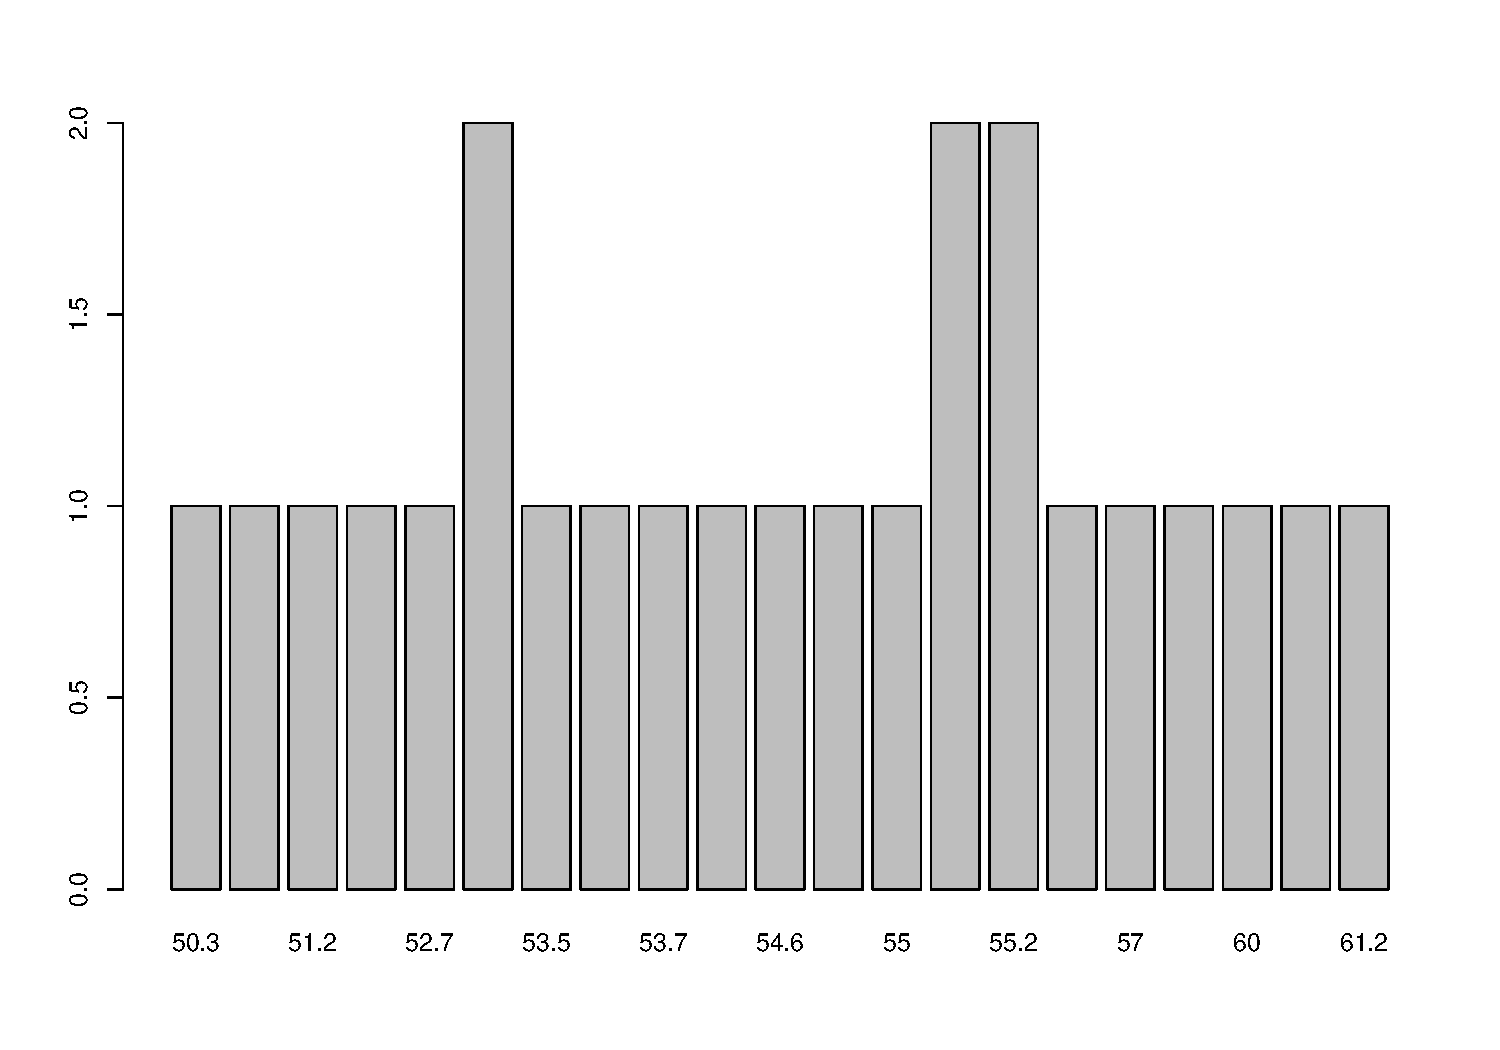
\includegraphics{Tema11.Distribuciones_probabilidad_files/figure-beamer/unnamed-chunk-2-1.pdf}

\end{frame}

\begin{frame}[fragile]{Distribución Geométrica}
\protect\hypertarget{distribuciuxf3n-geomuxe9trica-3}{}

El código de la distribución Geométrica:

\begin{itemize}
\tightlist
\item
  En \texttt{R} tenemos las funciones del paquete \texttt{Rlab}:
  \texttt{dgeom(x,\ prob),\ pgeom(q,\ prob),\ qgeom(p,\ prob),\ rgeom(n,\ prob)}
  donde \texttt{prob} es la probabilidad de éxito del experimento.
\item
  En \texttt{Python} tenemos las funciones del paquete
  \texttt{scipy.stats.geom}:
  \texttt{pmf(k,p),\ cdf(k,p),\ ppf(q,p),\ rvs(p,\ size)} donde
  \texttt{p} es la probabilidad de éxito del experimento.
\end{itemize}

\end{frame}

\begin{frame}{Distribución Hipergeométrica}
\protect\hypertarget{distribuciuxf3n-hipergeomuxe9trica}{}

Consideremos el experimento ``extraer a la vez (o una detrás de otra,
sin retornarlos) \(n\) objetos donde hay \(N\) de tipo A y \(M\) de tipo
B''. Si \(X\) es variable aleatoria que mide el ``número de objetos del
tipo A'', diremos que \(X\) se distribuye como una Hipergeométrica con
parámetros \(N,M,n\) \[X\sim \text{H}(N,M,n)\]

\begin{itemize}
\tightlist
\item
  El \textbf{dominio} de \(X\) será \(D_X = \{0,1,2,\dots,N\}\) (en
  general)
\item
  La \textbf{función de probabilidad} vendrá dada por
  \[f(k) = \frac{{N\choose k}{M\choose n-k}}{N+M\choose n}\]
\end{itemize}

\end{frame}

\begin{frame}{Distribución Hipergeométrica}
\protect\hypertarget{distribuciuxf3n-hipergeomuxe9trica-1}{}

\begin{itemize}
\tightlist
\item
  La \textbf{función de distribución} vendrá dada por \[F(x) = \left\{
  \begin{array}{cl}
     0 & \text{si } x<0 
  \\ \sum_{k=0}^xf(k) & \text{si } 0\le x<n
  \\ 1 & \text{si } x\ge n
  \end{array}
  \right.\]
\item
  \textbf{Esperanza} \(E(X) = \frac{nN}{N+M}\)
\item
  \textbf{Varianza}
  \(Var(X) = \frac{nNM}{(N+M)^2}\cdot\frac{N+M-n}{N+M-1}\)
\end{itemize}

\end{frame}

\begin{frame}{Distribución Hipergeométrica}
\protect\hypertarget{distribuciuxf3n-hipergeomuxe9trica-2}{}

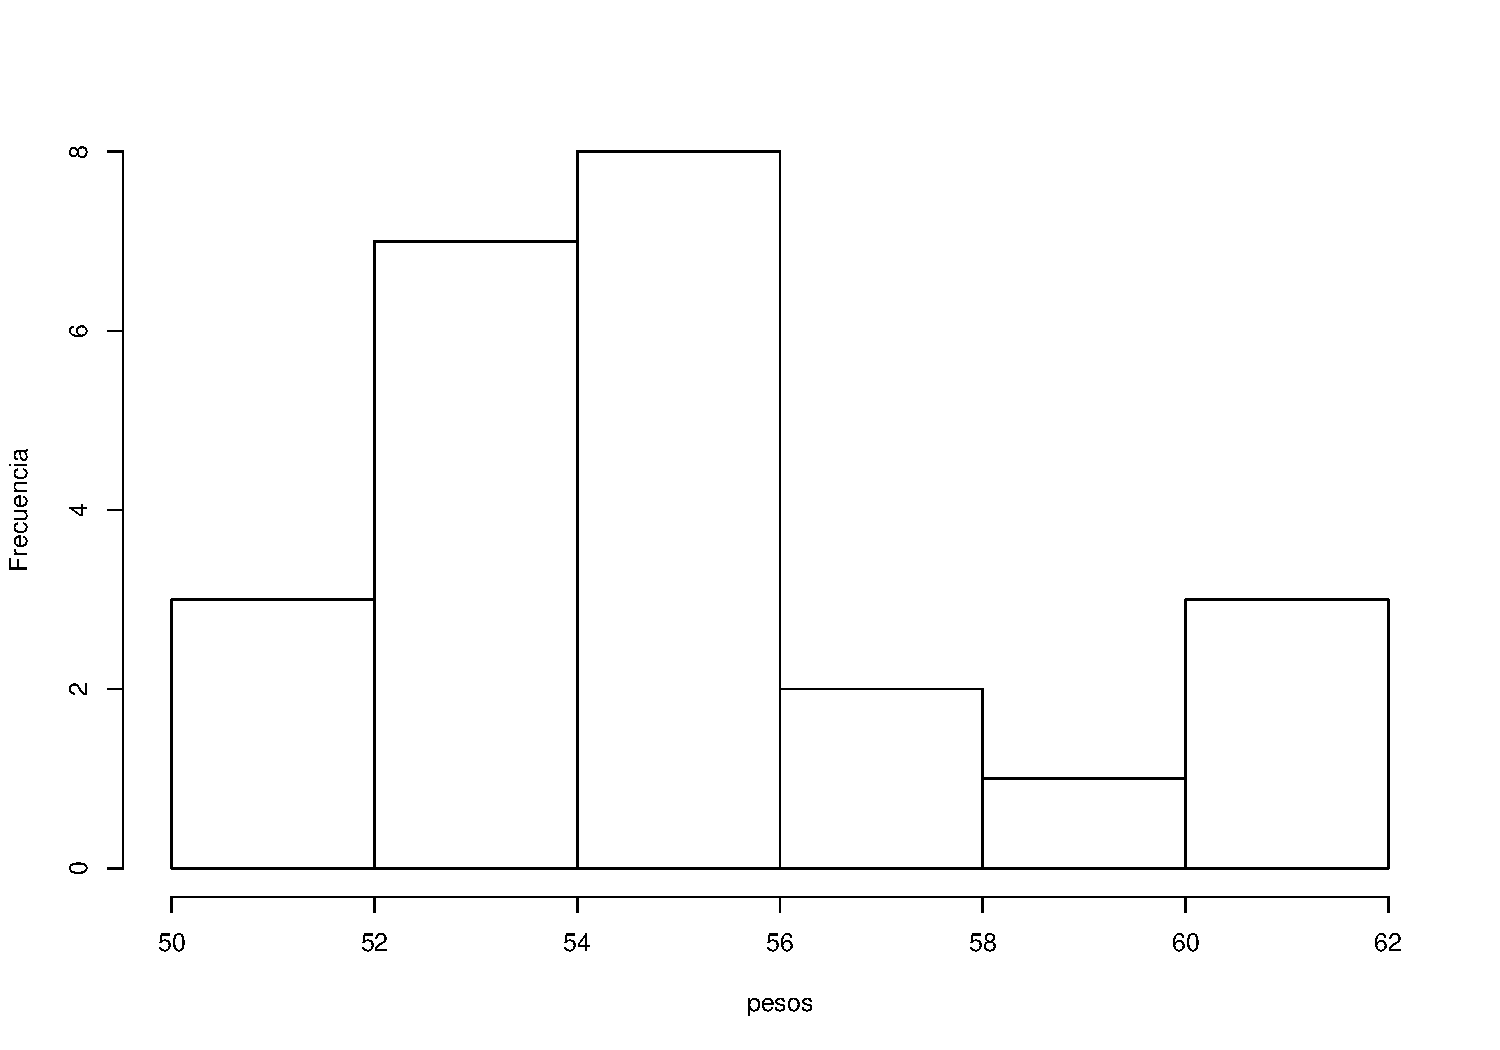
\includegraphics{Tema11.Distribuciones_probabilidad_files/figure-beamer/unnamed-chunk-3-1.pdf}

\end{frame}

\begin{frame}[fragile]{Distribución Hipergeométrica}
\protect\hypertarget{distribuciuxf3n-hipergeomuxe9trica-3}{}

El código de la distribución Hipergeométrica:

\begin{itemize}
\tightlist
\item
  En \texttt{R} tenemos las funciones del paquete \texttt{Rlab}:
  \texttt{dhyper(x,\ m,\ n,\ k),\ phyper(q,\ \ m,\ n,\ k),\ qhyper(p,\ \ m,\ n,\ k),\ rhyper(nn,\ \ m,\ n,\ k)}
  donde \texttt{m} es el número de objetos del primer tipo, \texttt{n}
  el número de objetos del segundo tipo y \texttt{k} el número de
  extracciones realizadas.
\item
  En \texttt{Python} tenemos las funciones del paquete
  \texttt{scipy.stats.hypergeom}:
  \texttt{pmf(k,M,\ n,\ N),\ cdf(k,M,\ n,\ N),\ ppf(q,M,\ n,\ N),\ rvs(M,\ n,\ N,\ size)}
  donde \texttt{M} es el número de objetos del primer tipo, \texttt{N}
  el número de objetos del segundo tipo y \texttt{n} el número de
  extracciones realizadas.
\end{itemize}

\end{frame}

\begin{frame}{Distribución de Poisson}
\protect\hypertarget{distribuciuxf3n-de-poisson}{}

Si \(X\) es variable aleatoria que mide el ``número de eventos en un
cierto intervalo de tiempo'', diremos que \(X\) se distribuye como una
Poisson con parámetro \(\lambda\)

\[X\sim \text{Po}(\lambda)\] donde \(\lambda\) representa el número de
veces que se espera que ocurra el evento durante un intervalo dado

\begin{itemize}
\item
  El \textbf{dominio} de \(X\) será \(D_X = \{0,1,2,\dots\}\)
\item
  La \textbf{función de probabilidad} vendrá dada por
  \[f(k) = \frac{e^{-\lambda}\lambda^k}{k!}\]
\end{itemize}

\end{frame}

\begin{frame}{Distribución de Poisson}
\protect\hypertarget{distribuciuxf3n-de-poisson-1}{}

\begin{itemize}
\tightlist
\item
  La \textbf{función de distribución} vendrá dada por \[F(x) = \left\{
  \begin{array}{cl}
     0 & \text{si } x<0 
  \\ \sum_{k=0}^xf(k) & \text{si } 0\le x<n
  \\ 1 & \text{si } x\ge n
  \end{array}
  \right.\]
\item
  \textbf{Esperanza} \(E(X) = \lambda\)
\item
  \textbf{Varianza} \(Var(X) = \lambda\)
\end{itemize}

\end{frame}

\begin{frame}{Distribución de Poisson}
\protect\hypertarget{distribuciuxf3n-de-poisson-2}{}

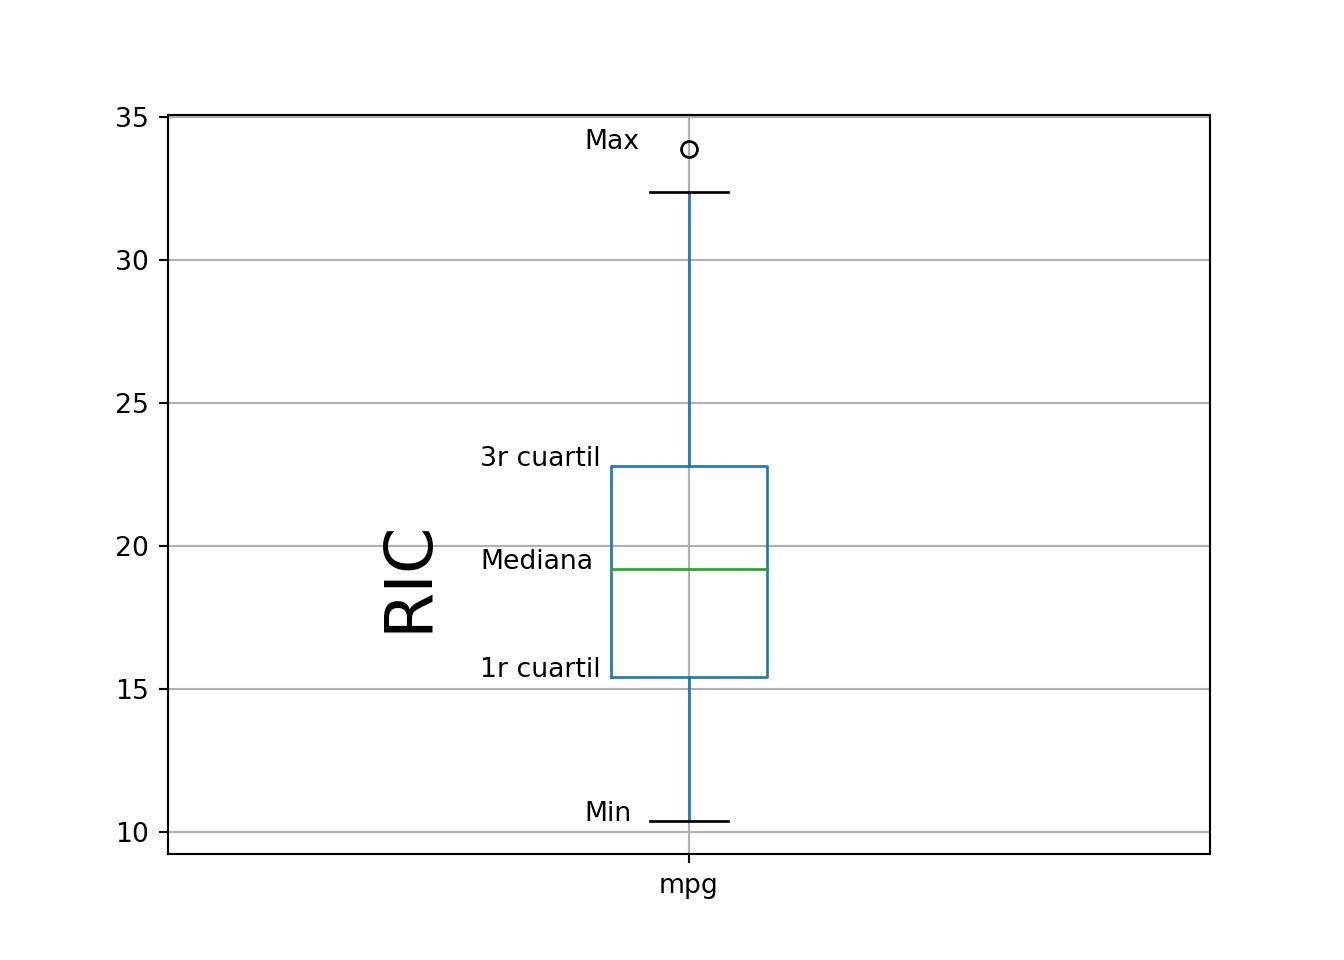
\includegraphics{Tema11.Distribuciones_probabilidad_files/figure-beamer/unnamed-chunk-4-1.pdf}

\end{frame}

\begin{frame}[fragile]{Distribución de Poisson}
\protect\hypertarget{distribuciuxf3n-de-poisson-3}{}

El código de la distribución de Poisson:

\begin{itemize}
\tightlist
\item
  En \texttt{R} tenemos las funciones del paquete \texttt{Rlab}:
  \texttt{dpois(x,\ lambda),\ ppois(q,lambda),\ qpois(p,lambda),\ rpois(n,\ lambda)}
  donde \texttt{lambda} es el número esperado de eventos por unidad de
  tiempo de la distribución.
\item
  En \texttt{Python} tenemos las funciones del paquete
  \texttt{scipy.stats.poisson}:
  \texttt{pmf(k,mu),\ cdf(k,mu),\ ppf(q,mu),\ rvs(M,mu)} donde
  \texttt{mu} es el número esperado de eventos por unidad de tiempo de
  la distribución.
\end{itemize}

\end{frame}

\begin{frame}{Distribución Binomial Negativa}
\protect\hypertarget{distribuciuxf3n-binomial-negativa}{}

Si \(X\) es variable aleatoria que mide el ``número de repeticiones
hasta observar los \(r\) éxitos en ensayos de Bernoulli'', diremos que
\(X\) se distribuye como una Binomial Negativa con parámetros \(r\) y
\(p\), \[X\sim\text{BN}(r,p)\] donde \(p\) es la probabilidad de éxito

\begin{itemize}
\tightlist
\item
  El \textbf{dominio} de \(X\) será \(D_X = \{r, r+1, r+2,\dots\}\)
\item
  La \textbf{función de probabilidad} vendrá dada por
  \[f(k) = {k-1\choose r-1}p^r(1-p)^{k-r}, k\geq r\]
\end{itemize}

\end{frame}

\begin{frame}{Distribución Binomial Negativa}
\protect\hypertarget{distribuciuxf3n-binomial-negativa-1}{}

\begin{itemize}
\tightlist
\item
  La \textbf{función de distribución} no tiene una expresión analítica.
\item
  \textbf{Esperanza} \(E(X) = \frac{r}{p}\)
\item
  \textbf{Varianza} \(Var(X) = r\frac{1-p}{p^2}\)
\end{itemize}

\end{frame}

\begin{frame}{Distribución Binomial Negativa}
\protect\hypertarget{distribuciuxf3n-binomial-negativa-2}{}

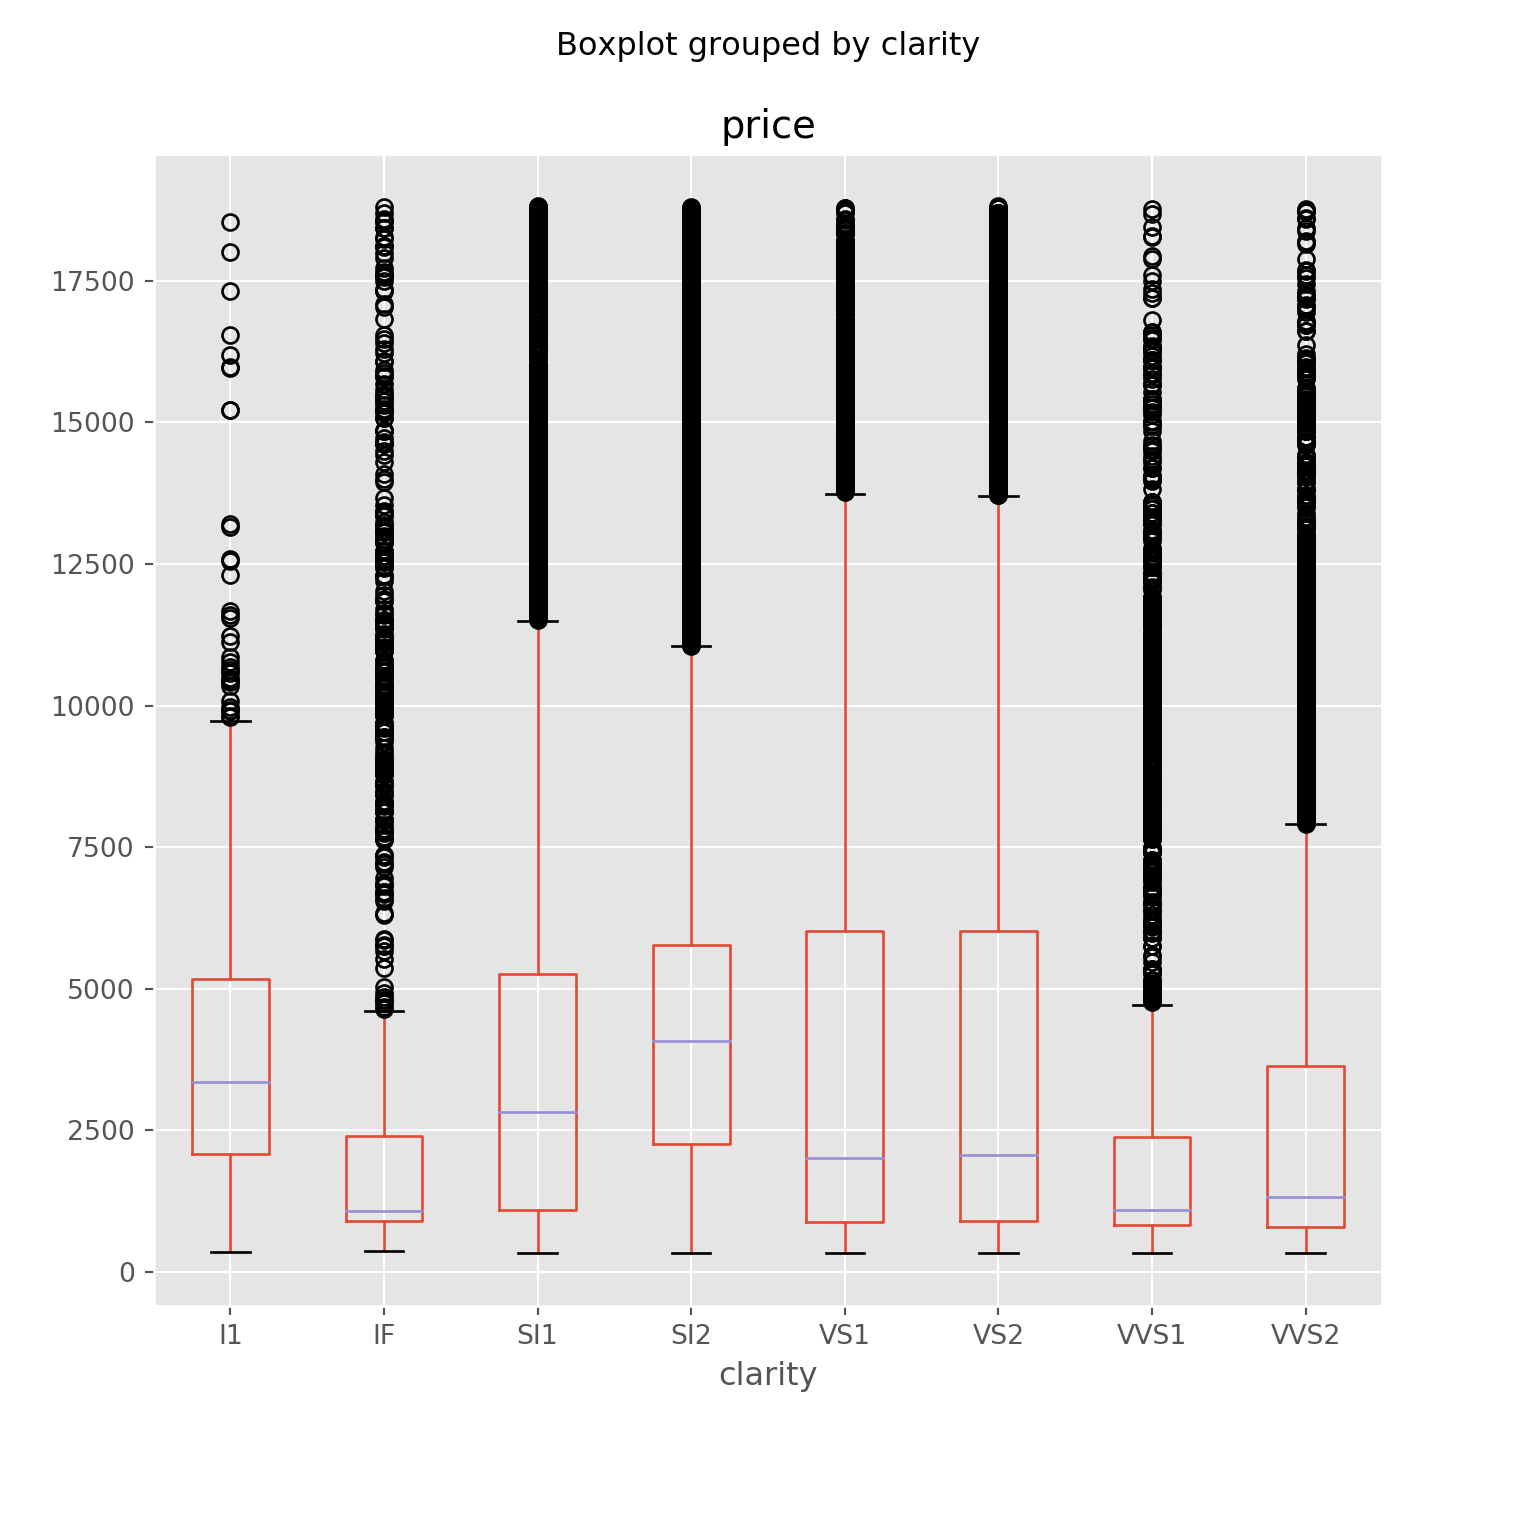
\includegraphics{Tema11.Distribuciones_probabilidad_files/figure-beamer/unnamed-chunk-5-1.pdf}

\end{frame}

\begin{frame}[fragile]{Distribución Binomial Negativa}
\protect\hypertarget{distribuciuxf3n-binomial-negativa-3}{}

El código de la distribución Binomial Negativa:

\begin{itemize}
\tightlist
\item
  En \texttt{R} tenemos las funciones del paquete \texttt{Rlab}:
  \texttt{dnbinom(x,\ size,\ prop),\ pnbinom(q,\ size,\ prop),\ qnbinom(p,\ size,\ prop),\ rnbinom(n,\ size,\ prop)}
  donde \texttt{size} es el número de casos exitosos y \texttt{prob} la
  probabilidad del éxito.
\item
  En \texttt{Python} tenemos las funciones del paquete
  \texttt{scipy.stats.nbinom}:
  \texttt{pmf(k,n,p),\ cdf(k,n,p),\ ppf(q,n,p),\ rvs(n,p)} donde
  \texttt{n}es el número de casos exitosos y \texttt{p} la probabilidad
  del éxito.
\end{itemize}

\end{frame}

\begin{frame}[fragile]{Distribuciones discretas en R}
\protect\hypertarget{distribuciones-discretas-en-r}{}

R conoce las distribuciones de probabilidad más importantes.

\begin{longtable}[]{@{}llll@{}}
\toprule
\begin{minipage}[b]{0.22\columnwidth}\raggedright
Distribución\strut
\end{minipage} & \begin{minipage}[b]{0.22\columnwidth}\raggedright
Instrucción en R\strut
\end{minipage} & \begin{minipage}[b]{0.22\columnwidth}\raggedright
Instrucción en Python\strut
\end{minipage} & \begin{minipage}[b]{0.22\columnwidth}\raggedright
Parámetros\strut
\end{minipage}\tabularnewline
\midrule
\endhead
\begin{minipage}[t]{0.22\columnwidth}\raggedright
Bernoulli\strut
\end{minipage} & \begin{minipage}[t]{0.22\columnwidth}\raggedright
\texttt{bern}\strut
\end{minipage} & \begin{minipage}[t]{0.22\columnwidth}\raggedright
\texttt{scipy.stats.bernoulli}\strut
\end{minipage} & \begin{minipage}[t]{0.22\columnwidth}\raggedright
probabilidad de éxito \(p\)\strut
\end{minipage}\tabularnewline
\begin{minipage}[t]{0.22\columnwidth}\raggedright
Binomial\strut
\end{minipage} & \begin{minipage}[t]{0.22\columnwidth}\raggedright
\texttt{binom}\strut
\end{minipage} & \begin{minipage}[t]{0.22\columnwidth}\raggedright
\texttt{scipy.stats.binom}\strut
\end{minipage} & \begin{minipage}[t]{0.22\columnwidth}\raggedright
tamaño de la muestra \(n\) y probabilidad de éxito \(p\)\strut
\end{minipage}\tabularnewline
\begin{minipage}[t]{0.22\columnwidth}\raggedright
Geométrica\strut
\end{minipage} & \begin{minipage}[t]{0.22\columnwidth}\raggedright
\texttt{geom}\strut
\end{minipage} & \begin{minipage}[t]{0.22\columnwidth}\raggedright
\texttt{scipy.stats.geom}\strut
\end{minipage} & \begin{minipage}[t]{0.22\columnwidth}\raggedright
probabilidad de éxito \(p\)\strut
\end{minipage}\tabularnewline
\begin{minipage}[t]{0.22\columnwidth}\raggedright
Hipergeométrica\strut
\end{minipage} & \begin{minipage}[t]{0.22\columnwidth}\raggedright
\texttt{hyper}\strut
\end{minipage} & \begin{minipage}[t]{0.22\columnwidth}\raggedright
\texttt{scipy.stats.hypergeom}\strut
\end{minipage} & \begin{minipage}[t]{0.22\columnwidth}\raggedright
\(N,M,n\)\strut
\end{minipage}\tabularnewline
\begin{minipage}[t]{0.22\columnwidth}\raggedright
Poisson\strut
\end{minipage} & \begin{minipage}[t]{0.22\columnwidth}\raggedright
\texttt{pois}\strut
\end{minipage} & \begin{minipage}[t]{0.22\columnwidth}\raggedright
\texttt{scipy.stats.poisson}\strut
\end{minipage} & \begin{minipage}[t]{0.22\columnwidth}\raggedright
esperanza \(\lambda\)\strut
\end{minipage}\tabularnewline
\begin{minipage}[t]{0.22\columnwidth}\raggedright
Binomial Negativa\strut
\end{minipage} & \begin{minipage}[t]{0.22\columnwidth}\raggedright
\texttt{nbinom}\strut
\end{minipage} & \begin{minipage}[t]{0.22\columnwidth}\raggedright
\texttt{scipy.stats.nbinom}\strut
\end{minipage} & \begin{minipage}[t]{0.22\columnwidth}\raggedright
número de éxitos \(r\) y probabilidad de éxito \(p\)\strut
\end{minipage}\tabularnewline
\bottomrule
\end{longtable}

\end{frame}

\hypertarget{variables-aleatorias-continuas}{%
\section{Variables aleatorias
continuas}\label{variables-aleatorias-continuas}}

\begin{frame}{Variable aleatoria continua}
\protect\hypertarget{variable-aleatoria-continua}{}

Variable aleatoria continua. Una v.a.
\(X:\Omega\longrightarrow\mathbb{R}\) es continua cuando su función de
distribución \(F_X:\mathbb{R}\longrightarrow[0,1]\) es continua

En este caso, \(F_X(x)=F_X(x^-)\) y, por este motivo,
\[p(X=x)=0\ \forall x\in\mathbb{R}\] pero esto no significa que sean
sucesos imposibles

\end{frame}

\begin{frame}{Función de densidad}
\protect\hypertarget{funciuxf3n-de-densidad}{}

Función de densidad. Función \(f:\mathbb{R}\longrightarrow\mathbb{R}\)
que satisface

\begin{itemize}
\tightlist
\item
  \(f(x)\ge 0\ \forall x\in\mathbb{R}\)
\item
  \(\int_{-\infty}^{+\infty}f(t)dt=1\)
\end{itemize}

Una función de densidad puede tener puntos de discontinuidad

\end{frame}

\begin{frame}{Variable aleatoria continua}
\protect\hypertarget{variable-aleatoria-continua-1}{}

Toda variable aleatoria \(X\) con función de distribución

\[F(x)=\int_{-\infty}^{x}f(t)dt\ \forall x\in\mathbb{R}\] para cualquier
densidad \(f\) es una v.a. continua

Diremos entonces que \(f\) es la función de densidad de \(X\)

A partir de ahora, considerareos solamente las v.a. \(X\) continuas que
tienen función de densidad

\end{frame}

\begin{frame}{Esperanza}
\protect\hypertarget{esperanza-1}{}

Esperanza de una v.a. continua. Sea \(X\) v.a. continua con densidad
\(f_X\). La esperanza de \(X\) es
\[E(X)=\int_{-\infty}^{+\infty}x\cdot f_X(x)dx\]

Si el dominio \(D_X\) de \(X\) es un intervalo de extremos \(a<b\),
entonces \[E(X)=\int_a^b x\cdot f_X(x)dx\]

\end{frame}

\begin{frame}{Esperanza}
\protect\hypertarget{esperanza-2}{}

Sea \(g:D_X\longrightarrow \mathbb{R}\) una función continua. Entonces,

\[E(g(X)) = \int_{-\infty}^{+\infty}g(x)\cdot f_X(x)dx\]

Si el dominio \(D_X\) de \(X\) es un intervalo de extremos \(a<b\),
entonces \[E(g(X))=\int_a^b g(x)\cdot f_X(x)dx\]

\end{frame}

\begin{frame}{Varianza}
\protect\hypertarget{varianza-2}{}

Varianza de una v.a. continua. Como en el caso discreto,
\[Var(X)=E((X-E(X))^2)\]

y se puede demostrar que

\[Var(X)=E(X^2)-(E(X))^2\]

\end{frame}

\begin{frame}{Desviación típica}
\protect\hypertarget{desviaciuxf3n-tuxedpica-1}{}

Desviación típica de una v.a. continua. Como en el caso discreto,
\[\sigma = \sqrt{Var(X)}\]

\end{frame}

\hypertarget{distribuciones-continuas-muxe1s-conocidas}{%
\section{Distribuciones continuas más
conocidas}\label{distribuciones-continuas-muxe1s-conocidas}}

\begin{frame}{Distribuciones continuas}
\protect\hypertarget{distribuciones-continuas}{}

\begin{itemize}
\tightlist
\item
  \href{https://es.wikipedia.org/wiki/Distribución_uniforme_continua}{Uniforme}
\item
  \href{https://es.wikipedia.org/wiki/Distribución_exponencial}{Exponencial}
\item
  \href{https://es.wikipedia.org/wiki/Distribución_normal}{Normal}
\item
  \href{https://es.wikipedia.org/wiki/Distribución_χ²}{Khi cuadrado}
\item
  \href{https://es.wikipedia.org/wiki/Distribución_t_de_Student}{t de
  Student}
\item
  \href{https://es.wikipedia.org/wiki/Distribución_F}{F de Fisher}
\end{itemize}

\end{frame}

\begin{frame}{Distribución Uniforme}
\protect\hypertarget{distribuciuxf3n-uniforme}{}

Una v.a. continua \(X\) tiene distribución uniforme sobre el intervalo
real \([a,b]\) con \(a<b\), \(X\sim\text{U}(a,b)\) si su función de
densidad es \[f_X(x)=\left\{
\begin{array}{rl}
     \frac{1}{b-a} & \text{si } a\le x\le b
  \\ 0 & \text{en cualquier otro caso}
\end{array}
\right.\]

Modela el elegir un elemento del intervalo \([a,b]\) de manera
equiprobable

\end{frame}

\begin{frame}{Distribución Uniforme}
\protect\hypertarget{distribuciuxf3n-uniforme-1}{}

\begin{itemize}
\item
  El \textbf{dominio} de \(X\) será \(D_X = [a,b]\)
\item
  La \textbf{función de distribución} vendrá dada por \[F_X(x)=\left\{
  \begin{array}{rl}
    0 & \text{si } x<a
  \\ \frac{x-a}{b-a} & \text{si } a\le x< b
  \\ 1 & \text{si } x\ge b
  \end{array}
  \right.\]
\item
  \textbf{Esperanza} \(E(X) = \frac{a+b}{2}\)
\item
  \textbf{Varianza} \(Var(X) = \frac{(b-a)^2}{12}\)
\end{itemize}

\end{frame}

\begin{frame}{Distribución Uniforme}
\protect\hypertarget{distribuciuxf3n-uniforme-2}{}

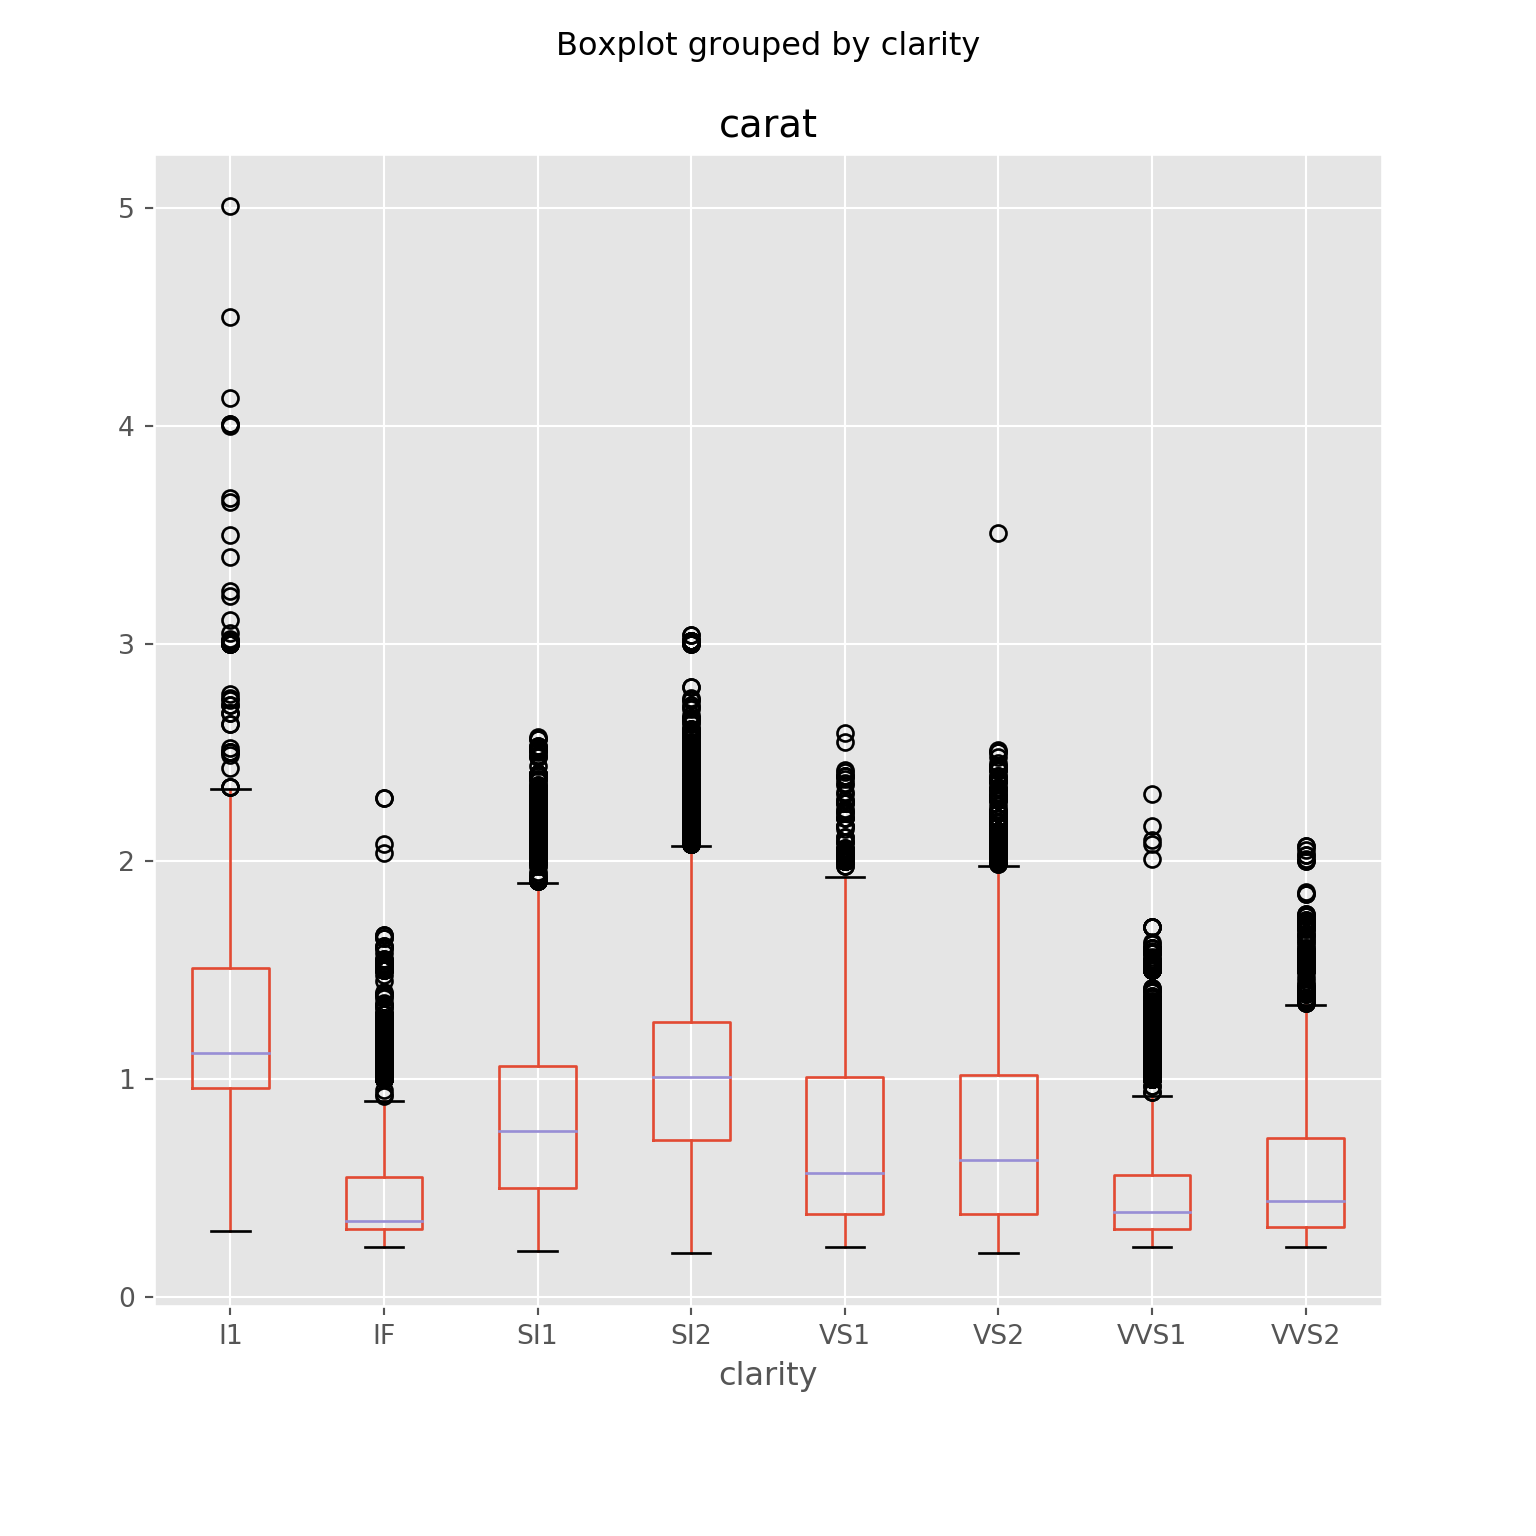
\includegraphics{Tema11.Distribuciones_probabilidad_files/figure-beamer/unnamed-chunk-6-1.pdf}

\end{frame}

\begin{frame}[fragile]{Distribución Uniforme}
\protect\hypertarget{distribuciuxf3n-uniforme-3}{}

El código de la distribución Uniforme:

\begin{itemize}
\tightlist
\item
  En \texttt{R} tenemos las funciones del paquete \texttt{stats}:
  \texttt{dunif(x,\ min,\ max),\ punif(q,\ min,\ max),\ qunif(p,\ min,\ max),\ runif(n,\ \ min,\ max)}
  donde \texttt{min} y \texttt{max} són los extremos de los intervalos
  de la distribución uniforme.
\item
  En \texttt{Python} tenemos las funciones del paquete
  \texttt{scipy.stats.uniform}:
  \texttt{pdf(k,loc,\ scale),\ cdf(k,loc,\ scale),\ ppf(q,loc,\ scale),\ rvs(n,loc,\ scaler)}
  donde la distribución uniforme está definida en el intervalo
  \texttt{{[}loc,\ loc+scale{]}}.
\end{itemize}

\end{frame}

\begin{frame}{Distribución Exponencial}
\protect\hypertarget{distribuciuxf3n-exponencial}{}

Una v.a. \(X\) tiene distribución exponencial de parámetro \(\lambda\),
\(X\sim\text{Exp}(\lambda)\), si su función de densidad es
\[f_X(x)=\left\{
\begin{array}{rl}
     0 & \text{si }  x\le 0
  \\ \lambda\cdot e^{-\lambda x} & \text{si }x>0
\end{array}
\right.\]

Teorema. Si tenemos un proceso de Poisson de parámetro \(\lambda\) por
unidad de tiempo, el tiempo que pasa entre dos sucesos consecutivos es
una v.a. \(\text{Exp}(\lambda)\)

Propiedad de la pérdida de memoria. Si \(X\) es v.a.
\(\text{Exp}(\lambda)\), entonces
\[p(X>s+t\ :\ X>s)=p(X>t)\ \forall s,t>0\]

\end{frame}

\begin{frame}{Distribución Exponencial}
\protect\hypertarget{distribuciuxf3n-exponencial-1}{}

\begin{itemize}
\item
  El \textbf{dominio} de \(X\) será \(D_X = [0,\infty)\)
\item
  La \textbf{función de distribución} vendrá dada por \[F_X(x)=\left\{
  \begin{array}{rl}
    0 & \text{si } x\le 0
  \\ 1-e^{-\lambda x} & \text{si } x>0
  \end{array}
  \right.\]
\item
  \textbf{Esperanza} \(E(X) = \frac{1}{\lambda}\)
\item
  \textbf{Varianza} \(Var(X) = \frac{1}{\lambda^2}\)
\end{itemize}

\end{frame}

\begin{frame}{Distribución Exponencial}
\protect\hypertarget{distribuciuxf3n-exponencial-2}{}

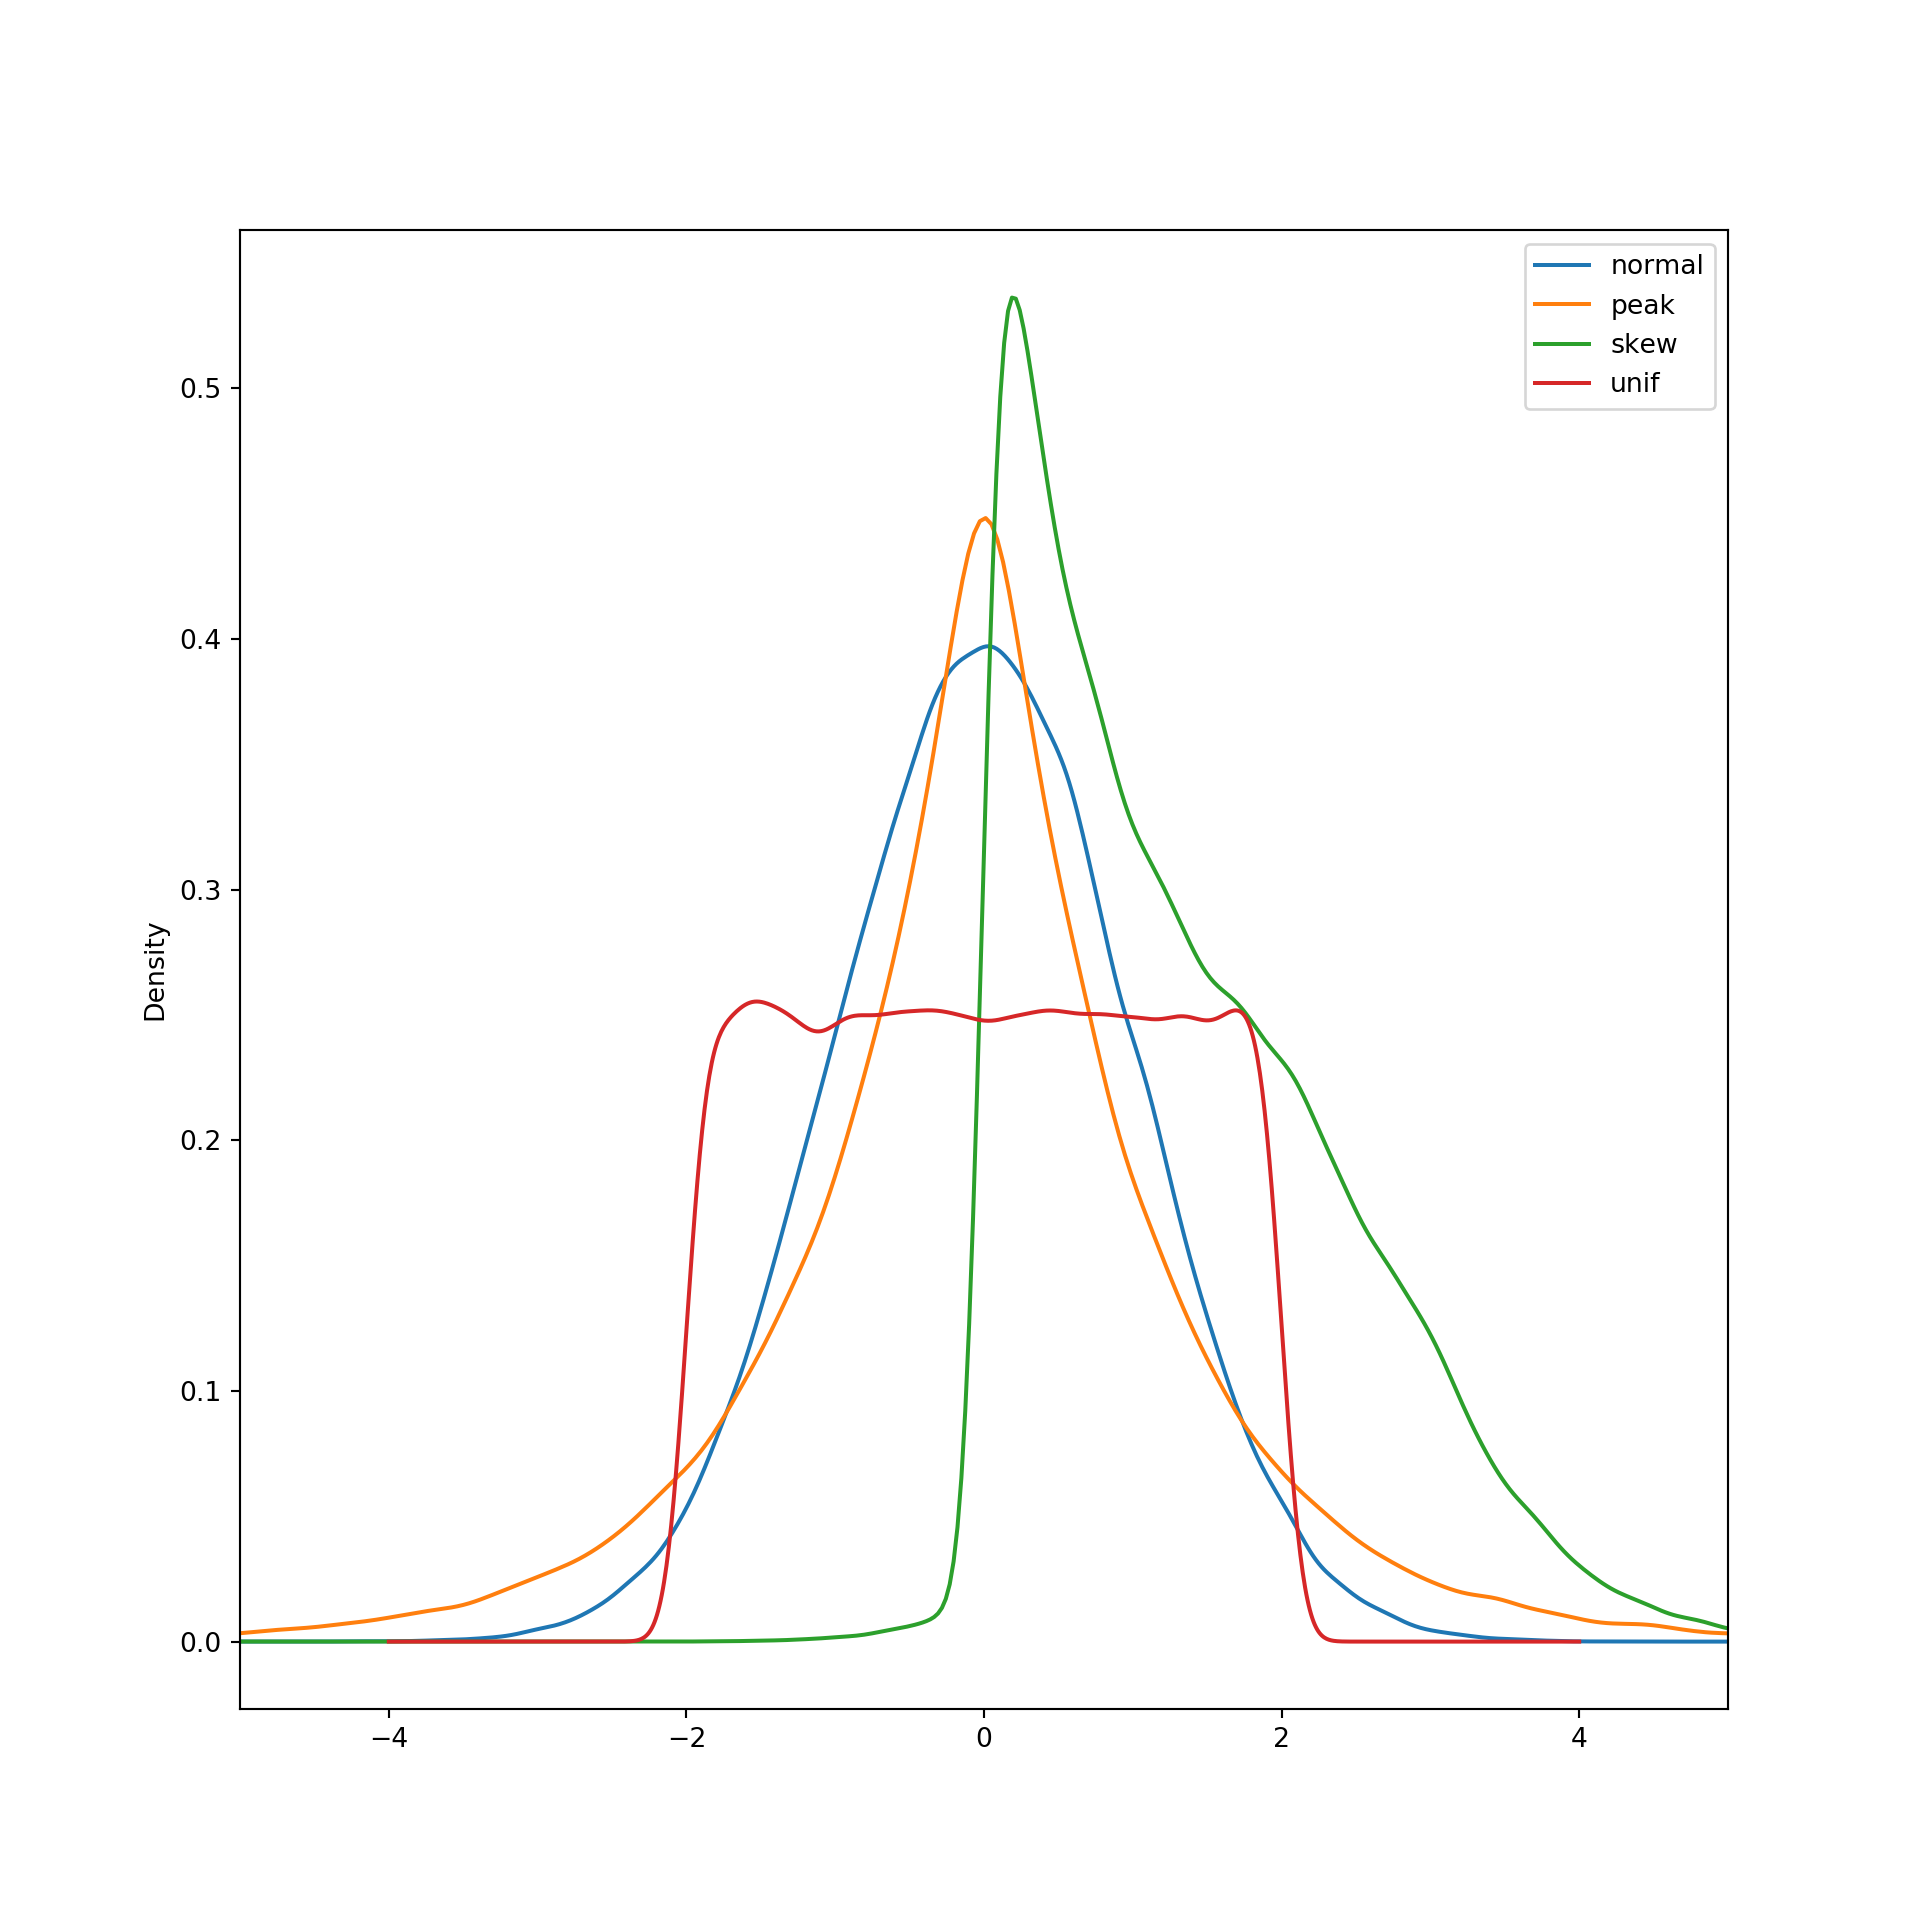
\includegraphics{Tema11.Distribuciones_probabilidad_files/figure-beamer/unnamed-chunk-7-1.pdf}

\end{frame}

\begin{frame}[fragile]{Distribución Exponencial}
\protect\hypertarget{distribuciuxf3n-exponencial-3}{}

El código de la distribución Exponencial:

\begin{itemize}
\tightlist
\item
  En \texttt{R} tenemos las funciones del paquete \texttt{stats}:
  \texttt{dexp(x,\ rate),\ pexp(q,\ rate),\ qexp(p,\ rate),\ rexp(n,\ \ rate)}
  donde \texttt{rate}\(=\lambda\) es el tiempo entre dos sucesos
  consecutivos de la distribución.
\item
  En \texttt{Python} tenemos las funciones del paquete
  \texttt{scipy.stats.expon}:
  \texttt{pdf(k,\ scale),\ cdf(k,\ scale),\ ppf(q,\ scale),\ rvs(n,\ scaler)}
  donde \texttt{scale}\(=1/\lambda\) es la inversa del tiempo entre dos
  sucesos consecutivos de la distribución.
\end{itemize}

\end{frame}

\begin{frame}{Distribución Normal}
\protect\hypertarget{distribuciuxf3n-normal}{}

Una v.a. \(X\) tiene distribución normal o gaussiana de parámetros
\(\mu\) y \(\sigma\), \(X\sim\mathcal{N}(\mu,\sigma)\) si su función de
densidad es
\[f_X(x)=\frac{1}{\sqrt{2\pi}\sigma}e^{-\frac{(x-\mu)^2}{2\sigma^2}}\quad \forall x\in\mathbb{R}\]

La gráfica de \(f_X\) es conocida como la Campana de Gauss

Cuando \(\mu = 0\) y \(\sigma = 1\), diremos que la v.a. \(X\) es
estándar y la indicaremos usualmente como \(Z\), la cual tendrá función
de densidad
\[f_Z(z)=\frac{1}{\sqrt{2\pi}}e^{-\frac{z^2}{2}}\quad \forall z\in\mathbb{R}\]

\end{frame}

\begin{frame}{Distribución Normal}
\protect\hypertarget{distribuciuxf3n-normal-1}{}

\begin{itemize}
\tightlist
\item
  \textbf{Esperanza} \(E(X) = \mu\)
\item
  \textbf{Varianza} \(Var(X) = \sigma^2\)
\end{itemize}

En particualr, si \(Z\) sigue una distribución estándar,

\begin{itemize}
\tightlist
\item
  \textbf{Esperanza} \(E(X) = 0\)
\item
  \textbf{Varianza} \(Var(X) = 1\)
\end{itemize}

\end{frame}

\begin{frame}{Distribución Normal}
\protect\hypertarget{distribuciuxf3n-normal-2}{}

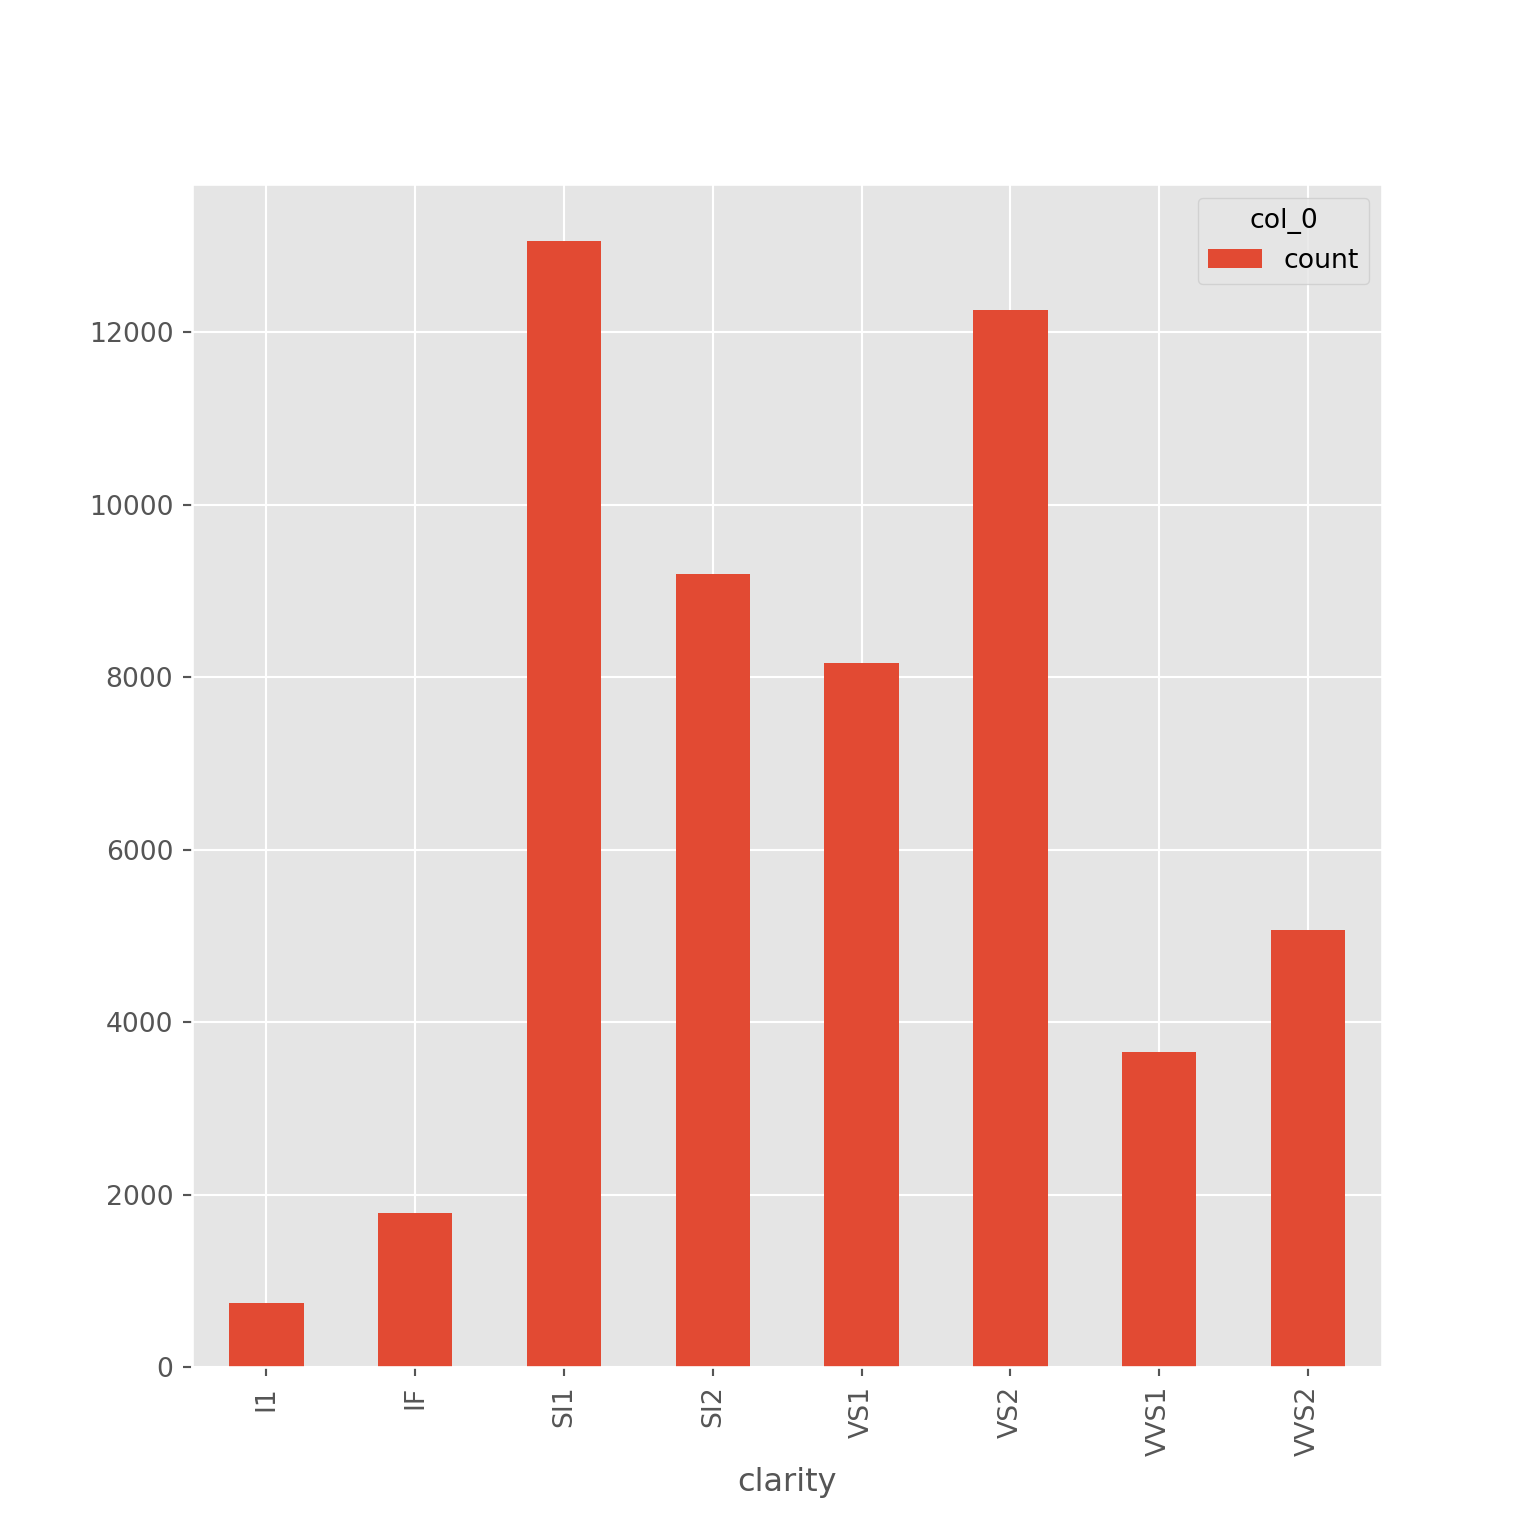
\includegraphics{Tema11.Distribuciones_probabilidad_files/figure-beamer/unnamed-chunk-8-1.pdf}

\end{frame}

\begin{frame}[fragile]{Distribución Normal}
\protect\hypertarget{distribuciuxf3n-normal-3}{}

El código de la distribución Normal:

\begin{itemize}
\tightlist
\item
  En \texttt{R} tenemos las funciones del paquete \texttt{stats}:
  \texttt{dnorm(x,\ mean,\ sd),\ pnorm(q,\ \ mean,\ sd),\ qnorm(p,\ \ mean,\ sd),\ rnorm(n,\ \ \ mean,\ sd)}
  donde \texttt{mean} es la media y \texttt{sd} es la desviación
  estándar de la normal \(N(\mu, \sigma)\).
\item
  En \texttt{Python} tenemos las funciones del paquete
  \texttt{scipy.stats.normal}:
  \texttt{pdf(k,\ mu,\ scale),\ cdf(k,\ \ mu,\ scale),\ ppf(q,\ \ mu,\ scale),\ rvs(n,\ \ mu,\ scale)}
  donde \texttt{mu} es la media y \texttt{scale} es la desviación
  estándar de la normal \(N(\mu, \sigma)\).
\end{itemize}

\end{frame}

\begin{frame}{Distribución Normal}
\protect\hypertarget{distribuciuxf3n-normal-4}{}

Estandarización de una v.a. normal. Si \(X\) es una v.a.
\(\mathcal{N}(\mu,\sigma)\), entonces
\[Z=\frac{X-\mu}{\sigma}\sim\mathcal{N}(0,1)\]

Las probabilidades de una normal estándar \(Z\) determinan las de
cualquier \(X\) de tipo \(\mathcal{N}(\mu,\sigma)\):

\[p(X\le x)=p\left(\frac{X-\mu}{\sigma}\le\frac{x-\mu}{\sigma}\right)=p\left(Z\le\frac{x-\mu}{\sigma}\right)\]

\end{frame}

\begin{frame}{Distribución Normal}
\protect\hypertarget{distribuciuxf3n-normal-5}{}

\(F_Z\) no tiene expresión conocida.

Se puede calcular con cualquier programa, como por ejemplo R, o bien a
mano utilizando las
\href{https://github.com/joanby/r-basic/blob/master/teoria/TablaNormal.pdf}{tablas
de la \(\mathcal{N}(0,1)\)}

Con las tablas se pueden calcular tanto probabilidades como cuantiles

\end{frame}

\begin{frame}[fragile]{Distribución Normal en R y Python}
\protect\hypertarget{distribuciuxf3n-normal-en-r-y-python}{}

Si a la hora de llamar a alguna de las 4 funciones siguientes:
\texttt{dnorm}, \texttt{pnorm}, \texttt{qnorm} o \texttt{rnorm} no
especificásemos los parámetros de la media ni la desviación típica, R
entiende que se trata de la normal estándar: la \(\mathcal{N}(0,1)\).

Es decir, R interpreta \(\mu = 0\) y \(\sigma = 1\)

En Python ocurre exactamente lo mismo.

\end{frame}

\begin{frame}{Otras distribuciones importantes}
\protect\hypertarget{otras-distribuciones-importantes}{}

\begin{itemize}
\tightlist
\item
  La distribución \(\chi^2_k\), donde \(k\) representa los grados de
  libertad de la misma y que procede de la suma de los cuadrados de
  \(k\) distribuciones normales estándar independientes:
\end{itemize}

\[X = Z_1^2 + Z_2^2+\cdots + Z_k^2\sim \chi_k^2\]

\end{frame}

\begin{frame}{Otras distribuciones importantes}
\protect\hypertarget{otras-distribuciones-importantes-1}{}

\begin{itemize}
\tightlist
\item
  La distribución \(t_k\) surge del problema de estimar la media de una
  población normalmente distribuida cuando el tamaño de la muestra es
  pequeña y procede del cociente
\end{itemize}

\[T = \frac{Z}{\sqrt{\chi^2_k/k}}\sim T_k\]

\end{frame}

\begin{frame}{Otras distribuciones importantes}
\protect\hypertarget{otras-distribuciones-importantes-2}{}

\begin{itemize}
\tightlist
\item
  La distribución \(F_{n_1,n_2}\) aparece frecuentemente como la
  distribución nula de una prueba estadística, especialmente en el
  análisis de varianza. Viene definida como el cociente
\end{itemize}

\[F = \frac{\chi^2_{n_1}/n_1}{\chi^2_{n_2}/n_2}\sim F_{n_1,n_2}\]

\end{frame}

\begin{frame}[fragile]{Distribuciones continuas en R}
\protect\hypertarget{distribuciones-continuas-en-r}{}

\begin{longtable}[]{@{}llll@{}}
\toprule
Distribución & Instrucción en R & Instrucción en Python &
Parámetros\tabularnewline
\midrule
\endhead
Uniforme & \texttt{unif} & \texttt{scipy.stats.uniform} & mínimo y
máximo\tabularnewline
Exponencial & \texttt{exp} & \texttt{scipy.stats.expon} &
\(\lambda\)\tabularnewline
Normal & \texttt{norm} & \texttt{scipy.stats.normal} & media \(\mu\),
desviación típica \(\sigma\)\tabularnewline
Khi cuadrado & \texttt{chisq} & \texttt{scipy.stats.chi2} & grados de
libertad\tabularnewline
t de Student & \texttt{t} & \texttt{scipy.stats.t} & grados de
libertad\tabularnewline
F de Fisher & \texttt{f} & \texttt{scipy.stats.f} & los dos grados de
libertad\tabularnewline
\bottomrule
\end{longtable}

\end{frame}

\begin{frame}{Otras distribuciones conocidas}
\protect\hypertarget{otras-distribuciones-conocidas}{}

\begin{itemize}
\tightlist
\item
  Distribución de Pareto (Power Law)
\item
  Distribución Gamma y Beta
\item
  Distribución Log Normal
\item
  Distribución de Weibull
\item
  Distribución de Cauchy
\item
  Distribución Exponencial Normal
\item
  Distribución Von Mises
\item
  Distribución Rayleigh
\item
  \ldots{}
\end{itemize}

\end{frame}

\end{document}
